\subsection{Formal Analysis}
\label{comesh:sec:analysis}

We formally analyze \sysname{}'s properties.
For the reader who wishes to skip this section, we  summarize  our findings:

\begin{itemize}
\item {\it Inheritance}: When a \kgroup{} %k-group 
changes, the state held by the old leader and new leader are identical.
\item {\it Safety}: No two routines that touch an overlapping set of devices, are allowed to execute simultaneously. 
\item {\it Liveness}: No routines deadlock.
\item {\it Progress}: Every routine makes progress.
\item We also calculate the (probabilistic) availability of the system when more than $f$ devices fail. 
\end{itemize}

\subsubsection{Inheritance}

\begin{definition}
Inheritance means that given a \kgroup{}, the old and new versions of the \kgroup{}---before and after epoch change, or after leader failure---maintain identical state. 
\end{definition}

For a device \kgroup{}, the state transferred to the new leader includes:
the device's current availability, and the lock queue. 
For a routine \kgroup{}, the new leader should receive: 
the routine state, and the IDs of devices already locked and released. 

\begin{lemma}
\label{comesh:lemma:inheritance}
Inheritance is guaranteed if at most one node fails during state transfer.
\end{lemma}

\begin{proof}
\label{comesh:lemma:inheritance:proof}
We consider two cases that trigger state transfer: 

\phantomsection
\label{comesh:lemma:inheritance:case1}
\noindent \textbf{Case 1--Leader Failure}:
Upon \kgroup{} leader $L_o$'s failure,
the new leader $L_n$ requests and receives from  all \kgroup{} members,  their local \kgroup{} state.
$L_n$ includes a(ny) state entry $e$ in the recreated state
if and only if there is at least 1 received state that contains $e$.
For the device \kgroups{},
every routine request in its lock queue is tagged with a sequence number
denoting when it reached $D_k$'s \kgroup{} leader--$L_n$ uses these to sort the queue. 
Since each routine entry $e$ in the lock queue was replicated
by at least a quorum of \kgroup{} members before the old leader $L_o$'s failure,
$L_n$ is guaranteed to receive the exact same set (and sequence) of routine requests as $L_o$.

\phantomsection
\label{comesh:lemma:inheritance:case2}
\noindent \textbf{Case 2--Epoch Change}:
New leader $L_n$ receives old leader $L_o$'s state. The single failure during state transfer may be:

\phantomsection
\label{comesh:lemma:inheritance:case2a}
\noindent \textbf{Case 2a--$L_o$ fails}:
$L_n$ detects $L_o$'s failure, and requests states from  all  old \kgroup{} members. This becomes Case~\hyperref[comesh:lemma:inheritance:case1]{1}. 

\phantomsection
\label{comesh:lemma:inheritance:case2b}
\noindent \textbf{Case 2b--$L_n$ fails}: A new leader $L_n'$ is elected (as per protocol) and requests state from $L_o$.

\phantomsection
\label{comesh:lemma:inheritance:case2c}
\noindent \textbf{Case 2c--member of old \kgroup{} fails}: This does not affect state transfer between $L_n$ and $L_o$. 

\phantomsection
\label{comesh:lemma:inheritance:case2d}
\noindent \textbf{Case 2d--member of new \kgroup{} fails}: 
A new node replaces the failed one, and it gets the new state from $L_n$. 
\end{proof}

\begin{lemma}
\label{comesh:lemma:inheritance:extension}
Inheritance is guaranteed if there are at most $\f{}$ node failures during state transfer.
\end{lemma}

\begin{proof}
\label{comesh:lemma:inheritance:extension:proof}
If either there are no epoch changes (\Cref{comesh:lemma:inheritance}: Case~\hyperref[comesh:lemma:inheritance:case1]{1}),  
or failures happen only among non-leader members during  epoch change
(\Cref{comesh:lemma:inheritance}~Cases: \hyperref[comesh:lemma:inheritance:case2c]{2c},~\hyperref[comesh:lemma:inheritance:case2d]{2d}),
each routine entry $e$ is maintained by at least $\f + 1 - \f = 1$ alive nodes.
Thus, \Cref{comesh:lemma:inheritance}: Case~\hyperref[comesh:lemma:inheritance:case1]{1} will recreate state correctly.

Upon epoch change, if old leader $L_o$ fails before  new leader $L_n$ gets  state,
$L_n$ (\Cref{comesh:lemma:inheritance}: Case~\hyperref[comesh:lemma:inheritance:case2a]{2a})  reconstructs the same state as $L_o$
since each state entry $e$ is maintained by at least $\f + 1 - \f = 1$ alive old \kgroup{} nodes. 
Repeated $L_n$ failures cause the new leader to re-attempt state reconstruction. 
 
If $L_n$ fails before $L_o$,  \Cref{comesh:lemma:inheritance}: Case~\hyperref[comesh:lemma:inheritance:case2b]{2b} applies.
\end{proof}

\subsubsection{\Safety{}}
\label{comesh:subsec:safety}

\begin{theorem}
\label{comesh:theorem:safety} {\bf [Safety]} 
No two routines that conflict in devices (i.e., their touched device sets are not disjoint) can execute simultaneously, under at most one node failure. 
\end{theorem}

\begin{proof}
\label{comesh:theorem:safety:proof}
Given routines $R_1, R_2$ that conflict in devices, we analyze OLA and SLA (\Cref{comesh:subsubsec:sla}) separately. 

\phantomsection
\label{comesh:theorem:safety:sla:proof}
\noindent {\bf \underline{SLA}: } 
Let $D_k$ be that shared device with the minimum $ID$. If $D_k$'s \kgroup{} leader $L_k$ does not fail, by definition, at most one routine can reach quorum
and therefore acquire the device lock.
During leader transition, all new requests are queued at the new leader $L_n$. Hence, we only discuss outstanding requests that have been approved when $L_k$ fails: 



\phantomsection
\label{comesh:theorem:safety:sla:case1}
\noindent \textbf{Case 1}: If $L_k$ fails before it has replicated the request
from $R_1$ to a quorum of \kgroup{} nodes,
$R_1$'s \kgroup{} leader resends $R_1$'s request after a timeout %T 
of not receiving an acknowledgment.

\phantomsection
\label{comesh:theorem:safety:sla:case2}
\noindent \textbf{Case 2}: If $L_k$ fails after replicating $R_1$'s request to a quorum in the \kgroup{},
new leader $L_n$ will receive $R_1$ from this  quorum. 

\phantomsection
\label{comesh:theorem:safety:sla:case3}
\noindent \textbf{Case 3}: If $L_k$ fails after $R_1$'s request reaches the top of the lock queue,
two sub-cases occur: (3a) Request approved by a quorum of nodes: 
new leader $L_n$ marks $R_1$ as the approved routine and notifies $R_1$'s \kgroup{} leader.
(3b) Request has not yet reached quorum:
$L_n$ adds $R_1$ to the lock queue.

\phantomsection
\label{comesh:theorem:safety:sla:case4}
\noindent \textbf{Case 4}: If $L_k$ fails after it has sent a Locked message to $R_1$'s \kgroup,
 $L_n$: 1) re-constitutes the lock queue from  surviving nodes,
and 2) (re)notifies $R_1$'s \kgroup{} leader of its approval.

{

\phantomsection
\label{comesh:theorem:safety:ola:proof}
\noindent {\bf \underline{OLA}:}
For a device $D_k$ touched by  $R_1$ \&  $R_2$, if $D_k$'s  \kgroup{}
leader $L_k$ does not fail, only one of $R_1, R_2$ can reach quorum and be approved to lock $D_k$. 
%
If $L_k$ fails, four cases arise:

\phantomsection
\label{comesh:theorem:safety:ola:case1}
\noindent \textbf{Case 1}: If $L_k$ fails before the quorum's pre-lock replication ack, new leader $L_n$ will have no record of it.  $R_1$'s \kgroup{} leader will resend the request after a timeout.


\phantomsection
\label{comesh:theorem:safety:ola:case2}
\noindent \textbf{Case 2}: If $L_k$ fails after quorum replication 
but before hearing back from $R_1$'s leader (to  lock for execution or release due to failed pre-lock),
$L_n$ will know $R_1$ has pre-locked $D_k$ from its group members, and resend pre-lock information back to $R_1$.


\phantomsection
\label{comesh:theorem:safety:ola:case3}
\noindent \textbf{Case 3}: If $L_k$ fails after hearing from $R_1$ (lock acquisition/releasing), but before getting a quorum acknowledgement, $R_1$'s \kgroup{} leader will resend the request after a timeout.


\phantomsection
\label{comesh:theorem:safety:ola:case4}
\noindent \textbf{Case 4}: If $L_k$ fails after it has locked $D_k$ and notifies $R_1$'s \kgroup{}
$L_n$: 1) re-constitutes the state from surviving nodes,
and 2) (re)notifies $R_1$'s \kgroup{} leader of its approval.
}
\end{proof}

\subsubsection{\Liveness{}}
\label{comesh:subsec:liveness}

\begin{theorem}
\label{comesh:theorem:deadlock} {\bf [No Deadlocks]} 
No routines deadlock.
\end{theorem}

\begin{proof}
\label{comesh:theorem:deadlock:proof:sla}
Each of SLA and OLA violate separate necessary conditions for deadlocks. 
SLA avoids ``wait for'' cycles among routines, since routines only wait for higher-$ID$ devices than they have already locked.
\phantomsection
\label{comesh:theorem:deadlock:proof:ola}
{
OLA violates the ``hold and wait'' condition since routines do not wait (and instead abort) for any already-locked devices. 
}
%
Leader change and failure do not affect device locks held by \sysname.
Meanwhile Lemmas~\ref{comesh:lemma:inheritance} and~\ref{comesh:lemma:inheritance:extension} guarantee inheritance.
Thus lock assignment is not influenced by leader changes and failures, i.e., there is no deadlock.
\end{proof}

The following theorem can be applied inductively. 
\begin{theorem}
\label{comesh:theorem:progress} {\bf [Progress/Liveness]} 
Consider a set of executing routines $\mathcal{R}$ 
still waiting to acquire 1 or more locks, and a set of devices $\mathcal{D}$ they are waiting for. If no further routines arrive into $\mathcal{R}$, and SLA is used for locking,  then: at least one routine from the set $\mathcal{R}$ will make progress (i.e., get access to one more device among the devices that it desires).
\end{theorem}
\begin{proof}
Consider the highest-$ID$ device $D$ in set $\mathcal{D}$, and the routine $R$ that currently holds the lock on $D$. $R$ cannot be waiting for any further locks (otherwise $D$ would not have the highest-$ID$ in $\mathcal{D}$). When $R$ eventually completes, the routine at the head of $D$'s queue will get access to $D$.
\end{proof}

For OLA, an adversary may always be able to prevent two competing routines from making progress. However, in practice, we observed that OLA makes fast progress. We use SLA as the default in the \sysname{} implementation.

\subsubsection{System Availability}
%Given \igt{$N$ total devices of which} 
Given $S$ \smart{}s, $G$ \kgroups{} each containing $k$ members, {and $F=$ total actual node failures during a run,}  we calculate the {\it availability} $P(\F{})$ =  
probability that \sysname{} still works correctly {under $F$ total failures,} i.e., all \kgroups{} contain $\ge (f+1)$ non-faulty nodes.

\begin{enumerate}
    \item When $\F{} \le \f{}$, $P(F) = 100\%$.
    \item When $\F{} > \f{}$, the {\it availability} is: 
        \begin{align*}
          P(F) &= P(\text{at most } f \text{ failures across all \kgroups)} \\
               &\;\ge\;1 - \sum_{i=1}^G P(> %\text{at least }
               f \text{ failures in one \kgroup}) \\
               &\;=\;1 - G \cdot \sum_{t=f+1}^{\min(k,F)}\frac{\binom{k}{t}\binom{S-k}{F-t}}{\binom{S}{F}}.
        \end{align*} 
\end{enumerate}


\noindent{$t$ counts the number of failures in a \kgroup{}, ranging from $(f+1)$ to $\min(k,F)$. The denominator counts all possible $F$ failures in the system.  The numerator's (i) left term counts all ways of selecting $t$ failures in a \kgroup{} of size $k$, and (ii) right term shows the selection of the remaining $(F-t)$ failures.  
}


\begin{figure}[t]
    \centering
    \begin{subfigure}[b]{0.48\linewidth}
        \centering
        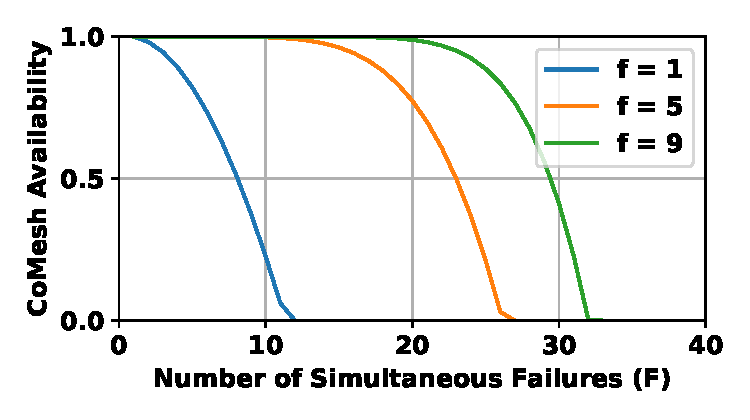
\includegraphics[width=\textwidth,alt={Line plot. x-axis: number of simultaneous failures F (0 to 40); y-axis: \sysname{} availability (0 to 1). Three inverse S-shaped curves for f=1 (blue), f=5 (orange), and f=9 (green), each holding at availability 1.0 and then dropping sharply to 0. The drop-off shifts right as f grows: f=1 falls around F=8 to 12, f=5 around F=20 to 27, and f=9 around F=28 to 32, so a larger f tolerates more simultaneous failures.}]{CoMesh/figures/analysis/pf_1_new.pdf}
        \caption{{\small \it Availability under different number of simultaneous failures.}}
        \label{comesh:subfig:prob-on-f}
    \end{subfigure}
    \hfill
    \begin{subfigure}[b]{0.5\linewidth}
        \centering
        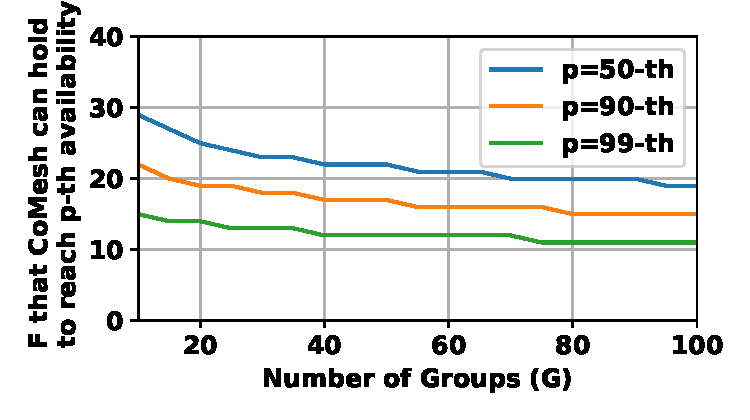
\includegraphics[width=\textwidth,alt={Line plot. x-axis: number of groups G (10 to 100); y-axis: the number of simultaneous failures F that \sysname{} tolerates while still meeting a target availability percentile (0 to 40). Three decreasing step curves: 50th percentile (blue, top) falls from about 29 to 19, 90th percentile (orange, middle) from about 22 to 15, and 99th percentile (green, bottom) from about 15 to 11. All decline as the number of groups grows and then flatten.}]{CoMesh/figures/analysis/pf_varyG_new.pdf}
        \caption{{\small \it Impact of different number of groups in the system ($f=5$).}}
        \label{comesh:subfig:prob-varyg}
    \end{subfigure}
    \caption{{\small \it Probability $P(F)$ of \sysname{} running correctly under different parameters. (Default $S=100$, $G=30, k=2f+1$.)}}
    \label{comesh:fig:prob-analysis}
    \medskip
\end{figure}

\Cref{comesh:fig:prob-analysis} plots this equation. Beyond $F>f$,
\Cref{comesh:subfig:prob-on-f} shows 
\sysname{} provides 50\% of availability when $\F{}$ grows as high as 2$\times f$. \Cref{comesh:subfig:prob-varyg} shows that to reach a specific percentile of availability $p$, \sysname{}'s tolerated $F$ drops very slowly, indicating scalability with the number of groups.
